\documentclass[preprint]{aastex}
\setlength{\textwidth}{6in}
\setlength{\textheight}{9in}
\setlength{\oddsidemargin}{0.0in}
\setlength{\parskip}{0.1mm}

\setlength{\topmargin}{-0.5in} % ... Matt's version
\citestyle{aa}
\usepackage{graphicx}
\usepackage[margin=1in]{geometry}
\usepackage{natbib}
\usepackage{epsfig}
\usepackage{amsmath}
\usepackage{color}     % added 26/12/2015
\usepackage{multicol}
%\usepackage{breqn}

% define some useful shortcuts:

% use in Math mode:

\newcommand{\rt}{{\bf r}_t}   % limb tangency point
\newcommand{\rsc}{{\bf r}_{\rm sc}}   %  space craft position wrt Saturn
\newcommand{\rsp}{{\bf r}_{\rm sc}'}   %  normalized space craft position 
\newcommand{\dpi}{\dot{\varpi}}    % apsidal rate (in eqns)
\newcommand{\dom}{\dot{\Omega}}    % nodal rate (in eqns)
\newcommand{\dpisec}{\dot{\varpi}_{\rm sec}} % secular apsidal rate (in eqns)
\newcommand{\domsec}{\dot{\Omega}_{\rm sec}} % secular nodal rate (in eqns)
\newcommand{\ares}{a_{\rm res}}    % resonant semimajor axis (in eqns)
\newcommand{\nres}{n_{\rm res}}    % resonant mean motion (in eqns)
\newcommand{\dd}{^\circ~{\rm d}^{-1}}   % deg/day 
\newcommand{\gcm}{{\rm g\,cm}^{-2}}   % g/cm2
\newcommand{\kms}{{\rm km\,s}^{-1}}   % km/s
\newcommand{\dasini}{a~\sin\Delta i}
\newcommand{\Bstar}{B_\ast}   % B_star
\newcommand{\nstar}{\hat{n}_\ast}   % n_star (unit vector)
\newcommand{\np}{{\bf n}_\ast'}   % normalized n_star (not a unit vector)
\newcommand{\half}{{1/2}}   % half-light level
\newcommand{\vperp}{v_\perp}   % perp . velocity
\newcommand{\Req}{R_{\rm eq}}    % equatorial radius
\newcommand{\Rpol}{R_{\rm pol}}    % polar radius
\newcommand{\tmin}{\tau_{\rm min}}    % minimum detectable optical depth
\newcommand{\tmax}{\tau_{\rm max}}    % maximum detectable optical depth

% use in Text mode:

\newcommand{\tdex}[1]{$\times 10^{#1}$}  % scientific notation (in text)
\newcommand{\microns}{$\mu$m}     % microns (in text)
\newcommand{\degrees}{$^\circ$}    % degrees (in text)
\newcommand{\Rs}{$R_S$}      % Saturn radii (in text)
\newcommand{\taun}{$\tau_{\rm n}$}   % tau_n (in text)
\newcommand{\fpat}{$\Omega_p$}     % pattern speed (in text)
\newcommand{\eg}{{\it e.g.,}}
\newcommand{\ie}{{\it i.e.,}}
\newcommand{\etal}{{\it et~al.}}
\newcommand{\beq}{\begin{equation}}
\newcommand{\eeq}{\end{equation}}
\newcommand{\Cas}{{\it Cassini}}
\newcommand{\Vgr}{{\it Voyager}}

% two column figures
\newenvironment{Figure}
  {\par\medskip\noindent\minipage{\linewidth}}
  {\endminipage\par\medskip}

\shorttitle{FINESST 2019 Proposal Andrew SD Foster}

\begin{document}
\section*{Personal Statement}
\vspace{-6mm}

\begin{multicols}{2}

\vspace{-3mm}
\subsection*{Research Experience}
\vspace{-3mm}

As an undergraduate at the University of Central Florida (UCF) I worked for Joe
Harrington for four years and earned BS degrees in Math and Physics. Joe's
group studies exoplanets using transit, secondary eclipse, and radial velocity
data.

My first year working with Joe, I used the group's orbits code (rv,
\citealp{CampoOrbit}) which fits orbital parameters to data from stellar radial
velocity measurements and transit and secondary eclipse timing using a Markov
chain. I used this code to fit an orbit to the planet TrES-1b \citep{tres1}. 

During my second and third years of working for Joe, I worked on a code called
Bayesian Atmospheric Radiative Transfer (BART, \citealp{BARTI}). BART uses a
Markov chain to constrain the atmospheres of hot-Jupiter exoplanets by fitting
the radiative transfer model described by \cite{RojoThesis} to transit and
secondary eclipse spectroscopy data. 

I optimized the radiative transfer model so it could run $10^5$ to $10^7$ times
within the Markov chain. Patricio Cubillos and I went through all 15,000+ lines
of code to determine what could be moved to an initialization function which
would be run first, and what would have to be looped over for every iteration.
After that, we used a code performance profiler to further optimize the runtime
of the code.

During my third rnd fourth years of working for Joe, I used our Photometry for
Orbits, Eclipses, and Transits (POET, \cite{StevensonPOET}) pipeline to fit a
light curve to two secondary-eclipse observations of the planet HAT-P-30b. A
companion star complicated this analysis, and I modified POET to be able to
model and subtract out the flux from this companion star. I then used our orbit
code to fit an orbit to HAT-P-30b.  Finally, I used BART to fit an atmosphere
to HAT-P-30b and published a first-author paper.  \citep{HAT30}.

\vspace{-3mm}
\subsection*{Outreach and Education Experience}
\vspace{-3mm}

At UCF, I ran the Astronomy Society. We held an open-to-the-public observing
event every week (weather permitting) at the UCF Robinson Observatory 8-inch
telescopes on the lawn and a tour inside of the observatory and its half-meter
telescope. We would give additional private events for groups such as scout
troops or local elementary schools in exchange for donations for our annual
science project, a stratospheric weather balloon launch.

In grad school at Cornell, I am the outreach coordinator for the graduate
students, organizing events at local libraries, the museum of the earth,
youth groups, and local 4-H groups. I have also assisted with outreach events
organized by Cornell's Spacecraft and Planetary Imaging Facility (SPIF).

I am in my sixth semester of being a graduate TA, including my second year
running a class of my own design. I adapted the UCF Astronomy Society's
stratospheric balloon project into an optional one credit lab class for our
intro to astronomy students.

In lab 1 the students propose designs for a weather balloon payload that fits
within a \$600 budget and 800g weight limit. The proposal includes constructing
a prototype of the structure of the payload from old styrofoam containers and
cardboard and writing a proposal for what electronics they want to use their
budget on.

In lab 2 the lab groups negotiate these multiple proposals down to a single
proposal within the timeframe of a single 2.5 hour lab session.

The third lab involves constructing and completing the payload, including
soldering and programming the electronics, performing drop tests to
determine the payload's terminal velocity, and learning to calculate
predicted landing sites using a program that integrates high altitude wind profiles.

The fourth lab is launch and recovery of the weather balloon.

\end{multicols}





\section*{Occultation Observations of Saturn with \Cas~VIMS}
%\author{Andrew SD Foster}
%\affil{Department of Astronomy, Cornell University, Ithaca NY 14853 }
\maketitle

\begin{multicols}{2}

\vspace{-9mm}
\section{Goals of the Investigation}
\vspace{-3mm}

During \Cas's 13 years in orbit around Saturn, the spacecraft's Visual and
Infrared Mapping Spectrometer (VIMS) performed over 100 stellar occultation
experiments on Saturn, covering a wide range of latitudes and seasons.
\cite{occpaperI} describe the VIMS campaign of occultations, including the
relevant instrumental setups for observing stellar and solar occultations,
event predictions, geometric and photometric calibrations, and instrumental
sensitivity. 

Occultation observations at different observer geometries and wavelengths probe
different levels of a planet's atmosphere. Spacecraft radio occultations are
sensitive to differential refraction \citep{Kliore04}, and probe the lower
stratosphere and upper troposphere of Saturn at pressures of a few mbar to
$\sim1$~bar \citep{Lindal85}.  Earth-based visible and near-infrared
occultations of the outer planets are also sensitive to differential refraction
and probe the upper stratosphere and mesosphere at pressures in the microbar
range \citep{ElliotVeverka76, Elliot79, French78}.  Spacecraft UV occultations
($\lambda < 150$~nm) are dominated by molecular and atomic absorption and probe
the thermosphere of Saturn at pressures in the nanobar to $\sim1~\mu$bar range
\citep{Broadfoot81, Sandel82, Smith83}.

This proposal deals with occultations observed by the \Cas~VIMS instrument,
which took time series of spectra with 20-40 ms sample rates at near-infrared
wavelengths ($0.88 - 5.1$~\microns\ in 256 spectral channels) as stars
disappeared behind Saturn. These data cover an intermediate regime where some
wavelengths are dominated by differential refraction and some by molecular
absorption (methane and ethane). They span pressures from $\sim20~\mu$bar to
$\sim5$~mbar, covering a large part of Saturn's stratosphere. See figure
\ref{fig:datasample} for an example of what a VIMS occultation looks like.

Modeling the effects of differential refraction reveals the temperature profile
of the atmosphere. Modeling the effects of molecular absorption reveals the
composition. This data is the first that allows us to retrieve both
simultaneously from the same \Cas~dataset and in the same region of the atmosphere.

The principle goals of observing Saturn stellar occultations with VIMS were to
obtain light curves that could be inverted to obtain temperature-pressure
profiles of the planet's stratosphere, and to obtain vertical profiles of
CH$_4$ abundance in the upper stratosphere with which to test photochemical and
eddy-diffusion models such as those of \cite{Moses00} and \cite{Moses05}. Some
preliminary results have been presented by \cite{Nicholson06} and
\cite{Banfield11}, but so far no comprehensive study has been completed or
published.

{\bf I propose to perform just such a comprehensive study that will attempt to
answer the questions outlined in the previous paragraph and to address the NASA
Planetary Science Research Program SMD 2014 Science Plan top-level goal to:

``Advance the understanding of how the chemical and physical processes in the Solar System
operate, interact and evolve."

More specifically, we will address the topic:

``Investigate the origins, evolution, and properties of the atmospheres of
planetary bodies (including satellites, small bodies, and exoplanets)" 

as well as

``Enhance the scientific return of NASA Planetary Science Division missions
through the analysis of data collected by those missions" }

\begin{figure*}[ht]
\centering
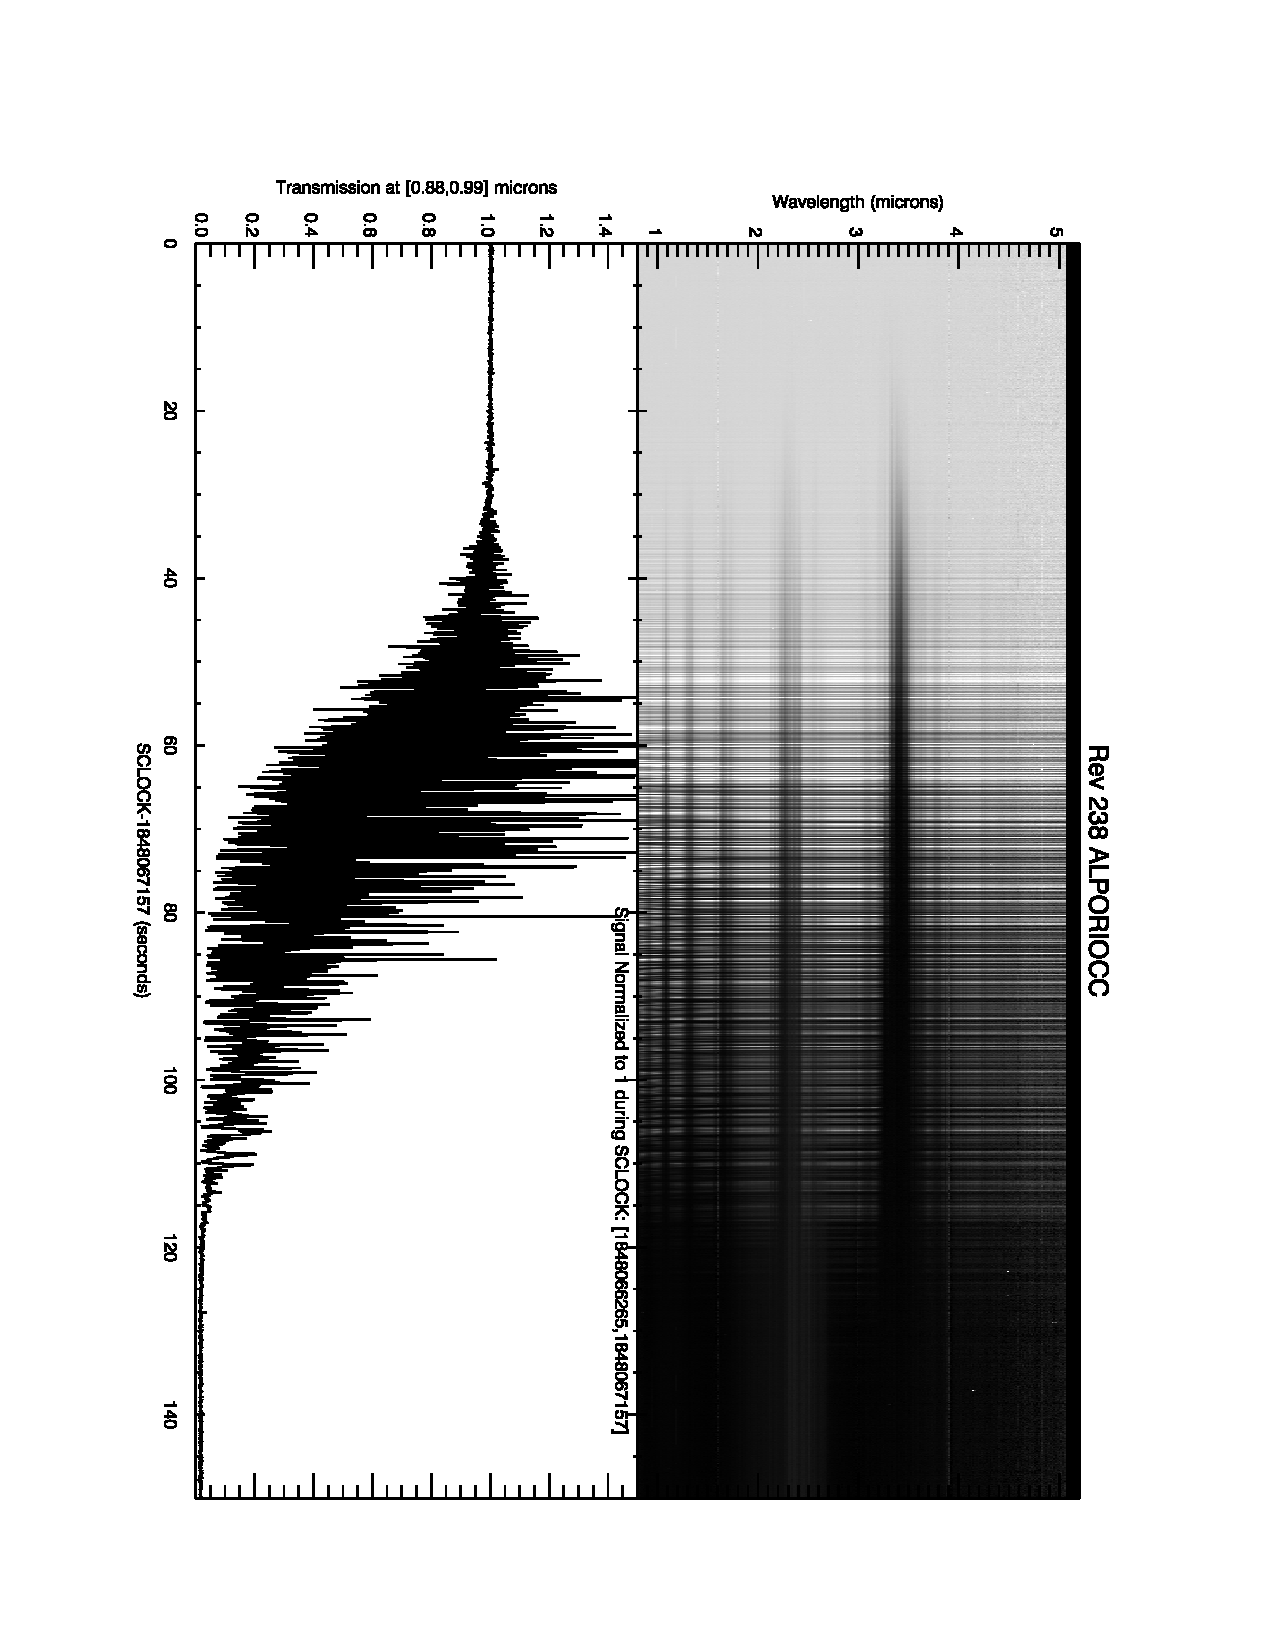
\includegraphics[angle=90, width=\textwidth]{./figs/alporiocc238_atmov_072517.pdf}

\caption{
\footnotesize
Occultation of $\alpha$~Orionis during Cassini rev: 238 at planetocentric
latitude $-64.9^\circ$ from a range of $959,000$~km with an integration time of
20~ms.{\bf Upper panel} shows stellar signal with wavelength increasing
vertically and time increasing horizontally. Stellar signal drops due to
differential refraction independently of wavelength except for the molecular
absorption in the narrow horizontal bands at 3.4, 2.3, 1.7, 1.4, 1.1 and
0.9~\microns.  {\bf The lower panel} shows the flux averaged between 0.9 and
1.0~\microns where molecular extinction is unimportant. In both panels, the
stellar flux is normalized to unity in the period prior to the occultation. 
}

\label{fig:datasample}
\end{figure*}

\vspace{-9mm}
\section{Scientific Significance}
\vspace{-3mm}

Pre-\Cas~observations of Saturn's temperature show a peak in seasonal variation
at around 3 mbar \citep{Yanamandra2005}, the
region that the VIMS stellar occultation data probe.  CIRS observations by
\cite{Flasar2004, Flasar2005, Fletcher2007} 
confirm this. Our proposed analysis can provide far better altitude resolution
than the CIRS results in this critical region. Furthermore, the CIRS results
are derived from thermal emission in the methane band at 8\microns and cannot
easily disentangle variations in temperature from variations in methane mixing
ratio.  We expect methane abundances also to depend on latitude and season as
described by \cite{Moses05} and \cite{Fouchet09}.  The proposed analysis will
allow us to recover temperature profiles and methane abundances {\it
independently of each other} at various latitudes and at seasons spanning
almost half of a Saturnian year. {\bf (Science Project 1: Verify CIRS Results)}

The chemical abundance profiles calculated in \cite{Moses05} match the "methane
cycle" described in \cite{Strobel69}. Methane diffuses up through the
stratosphere to the homopause, slowly dropping in abundance through the region
of the stratosphere to which VIMS occultations are sensitive. Far above this
region of the stratosphere, methane undergoes photodissociation and is
converted to higher-order hydrocarbons which diffuse back down to the
troposphere where they are converted back to methane. The gases diffuse from
their source to their sink via turbulence- or wind-driven eddy diffusion. The
rates of diffusion, production, and destruction of these gases determine the
shape of the abundance profiles through the stratosphere seen in figure
\ref{fig:MosesPlot}.

\begin{figure*}[ht]
\centering
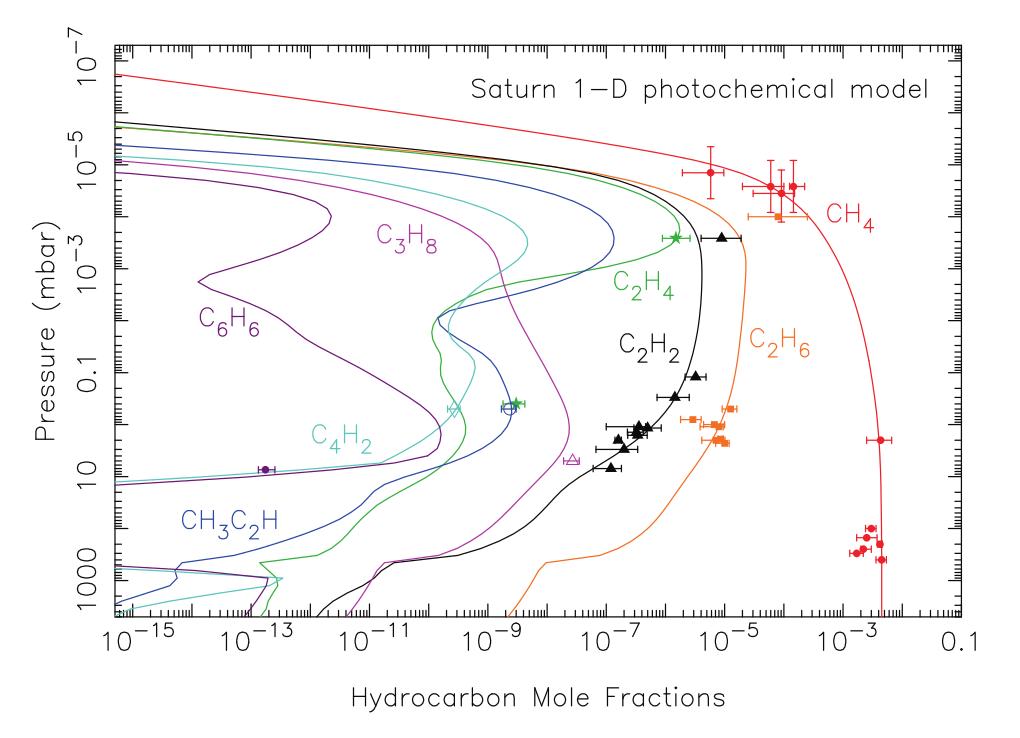
\includegraphics[width=\linewidth]{./figs/Fouchet09.png}

\caption{
\footnotesize
Figure taken from \cite{Fouchet09}. Hydrocarbon mole fractions as a function of
pressure in Saturn's upper atmosphere as derived from the "Model C" 1-D
steady-state photochemical model of \cite{Moses05}. The solid curves represent
the model profiles for the individual hydrocarbons (as labeled), and the
symbols with associated error bars represent current infrared and ultraviolet
observations. Methane is created in the troposphere and diffuses upwards to the
homopause and the thermosphere where it is photochemically destroyed. Ethane
and acetylene are produced at around \tdex{-4} mbar and diffuse down to the
troposphere where they are converted back to methane. This is the methane cycle
described in \cite{Strobel69}
}

\label{fig:MosesPlot}
\end{figure*}

As noted by \cite{Fouchet09}, important byproducts of these multiple profiles
will be a better determination of the altitude of the CH$_4$ homopause on
Saturn (which is known to be quite variable with latitude from UV occultations
\citealp{Koskinen13, Koskinen15}). This is a function of the rate of
photochemistry, which destroys CH$4$ in the upper atmosphere \citep{Fouchet09},
and the speed of zonal winds in the stratosphere which distort the shape of the
planet through the centrifugal force \citep{Merritt19}.  {\bf (Science Project
2: Measure the Homopause)}

Photodissociated methane is partially converted into ethane on its way to
becoming aerosols composed of higher order hydrocarbons. Chemical abundances in
the stratosphere impact the thermal profile of the entire atmosphere since
trace gasses are the major absorbers of radiation from the sun and Saturn's
blackbody emissions from lower levels. The proposed analysis will constrain
both the methane and ethane mixing ratios, giving us insight into seasonal
variations in photochemistry and eddy-diffusion rates that we can compare to
models such as those described in \cite{Moses05}. {\bf (Science Project 3: 
Test Models of Chemistry and Eddy-Diffusion)}

Photochemistry also leads to aerosol production. Although not very spectrally
active in our observations, aerosols are thought to be chemically important as
a factor in cloud formation because they sediment downwards to serve as
cloud-condensation nuclei for condensible volatiles in the troposphere
\citep{Fletcher18}. We will constrain photochemistry and eddy-diffusion rates
through a direct measurement of the relative mixing ratios of methane to
ethane, which will help future investigators understand aerosol production in
the thermosphere and cloud formation processes in the convective regions of the
troposphere. We will measure these abundances with high radial resolution over
the course of nearly half of a Saturnian year at a multitude of latitudes
thanks to \Cas's long-lasting mission in the Saturn system.

Finally, uncertainties in the production and optical properties of
photochemical haze are a major stumbling blocks in current hot-Jupiter
exoplanet atmospheric models and retrievals, as they are thought to be the
cause of the flattening of the transit spectra of gaseous exoplanets
\citep{Fraine13}.  Through providing a ground-truth
understanding of the atmosphere of one of our local giant planets whose
atmospheric chemistry is also photochemically driven, our analysis will help
future studies constrain the atmospheres of these exciting bodies that we will
soon be able to probe in greater detail with the James Webb Space Telescope,
ELT-class ground-based telescopes, and other future telescopes.

\vspace{-9mm}
\section{Technical Background}

\vspace{-3mm}
\subsection{Differential Refraction}
\vspace{-3mm}

Consider a light ray from the occulted star incident on a spherical planet of
radius $R$, at an impact parameter $\rho$. As it penetrates more deeply into
the atmosphere, where the refractive index of the gas is larger, the ray
gradually refracts towards the planet's center until it reaches a minimum
radius, after which it traces a mirror-image path back out of the atmosphere.  

The formal expression for the overall angular deflection of the ray once it
emerges from the atmosphere is:

\beq 
 \theta(\rho) = -2\rho \int_{r_0}^\infty \frac{dn/dr}{n\sqrt{n^2r^2 - \rho^2}}\, dr,
\label{eq:bending_angle}
\eeq

\noindent where $n(r)$  is the refractive index profile of the atmosphere,
and the ray's minimum radius $r_0$ is specified by the condition $n(r_0)r_0 = \rho$.

Adjacent light rays are deflected by progressively larger amounts as $\rho$
decreases and the rays penetrate more deeply into the atmosphere. As a result
of this {\it differential refraction}, the flux of light from the source is
reduced by a factor of $\Phi$:

\beq 
 \Phi(\rho) = \left( 1 - D\frac{d\theta}{d\rho} \right)^{-1}\left( 1 - \frac{D\theta}{\rho} \right)^{-1},
\label{eq:iso_flux}
\eeq

\noindent where $D$ is the distance from the planet to the observer. The second
factor represents the focusing effect that occurs near the center of the
geometric shadow and can be neglected for our data where $D\theta\ll\rho$.

{\bf As described in \cite{Elliot77} and \cite{French78}, we can use these two
expressions to perform an inverse Abel transform and invert our occultation
lightcurves in regions of the spectra dominated by differential refraction to
acquire multiple radial profiles of the temperature and pressure in the
planet's stratosphere.} 

This technique is standard for inversions of differential-refraction dominated
stellar occultations.  Due to Saturn's highly oblate shape, the above
expressions are adjusted in practice to use a local spherical fit to the
atmosphere.

We are confident that the attenuation of the starlight at wavelengths where
hydrocarbon molecular absorption is negligible is dominated by the
above-described impact of differential refraction and not aerosol-driven
scattering extinction. Although aerosols are an important chemical component of
Saturn's atmosphere, these particles are likely sub-micron in size and their
scattering efficiency should decrease rapidly with decreasing wavelength,
perhaps scaling as $\lambda^{-q}$ where $q$ is between 1 and 4. The aerosols on
Titan follow such a power law with $q\simeq1.8\pm0.5$ \citep{Bellucci09}. The
extinction in the VIMS Saturn occultations at wavelengths outside of the strong
hydrocarbon bands is observed to be essentially {\sl independent} of
wavelength, strongly suggesting that aerosol extinction is negligible at the
few mbar level and above and therefore we may neglect them in our models.

\vspace{-9mm}
\subsection{Morphology of an Occultation}
\vspace{-3mm}

Let's examine equation \ref{eq:iso_flux}, neglect the second term, and
substitute the appropriate isothermal expression for $\theta(\rho)$ to get an
approximate expression of $\Phi(\rho)$ that can give us some intuition for how
flux is lost over the course of an occultation:

\beq
 \Phi(\rho) \simeq \left( 1 + \frac{D\theta}{H} \right)^{-1}.
\label{eq:approx_flux}
\eeq

\noindent where the atmosphere's scale height $H = {\cal R}T/\mu g$, $T$ is the
temperature, $\mu$ is the mean molecular weight, $g$ is the local gravitational
acceleration, and ${\cal R}$ is the universal gas constant.

Note that $\Phi(\rho) \simeq \frac{1}{2}$ when $D\theta = H$, indicating that
the impact parameter for which the flux from the source has halved is dependent
on the distance to the observer $D$. This is the reason that Earth-based
stellar occultations probe much higher atmospheric levels than do those
observed by orbiting spacecraft at similar wavelengths. For typical VIMS
Saturn occultations, the refractive half-light level is at $p \sim 3$~mbar,
assuming that $\bar{T}_{stratosphere} \sim 140$K. 

The bending angle $\theta$ scales with the refractivity at the point of deepest
penetration of the ray which increases exponentially with depth, so the
attenuation of the rays increases rapidly as they drop below the half-light
level. However, the observed brightness of the occulted star falls off much
more gradually because the light rays are also deflected further into the
planet's geometric shadow, prolonging the star's visibility. The result is that
such a purely-refractive lightcurve has a long tail that extends well beyond
the half-light time. In our observations this tail is truncated because the
image of the star is refracted out of the single $0.25\times0.5$~mrad VIMS
pixel, leading to a "floor" beyond which we cannot probe. This occurs at
$\Phi\simeq\frac{1}{3.5}$, for $\theta\simeq0.25$~mrad, $D\simeq5$\tdex{5}~km,
and $H\simeq50$~km. This is empirically confirmed by a small number of VIMS
occultations observed in the instrument's imaging-mode, which has a larger
field-of-view at the expense of less-frequent time-sampling.

\vspace{-9mm}
\subsection{Molecular Absorption}
\vspace{-3mm}

Let's consider an "onion-skin" model of an atmosphere for which each thin
radial layer is of uniform composition and density. As a ray of star light
passes through each of these layers, it is attenuated according to the
equation:

\beq
\Phi(\lambda) = \Phi_0\ e^{-\delta\tau(\lambda)},
\label{eq:abs_flux}
\eeq

\noindent where $\Phi_0$ is the attenuation experienced before entering that layer
and $\delta\tau(\lambda)$ is the optical depth of the layer as a function of
wavelength, described by the equation:

\beq
\delta\tau(\lambda) = \kappa(\lambda) L d
\label{eq:optical_depth}
\eeq

\noindent Here, $\kappa$ is the absorption coefficient, $L$ is the slant
pathlength, and $d$ is the density of the layer which is known from the
inversion of the lightcurve at the refraction-dominated continuum wavelengths.

The data for a given occultation can be thought of as a time-series of spectra,
each of which cuts a deeper path through the atmosphere than its predecessor.
Each time-step can be used to constrain the opacity of an additional deeper
layer, and then be used as an input to the next timestep since that layer will
also be probed during the subsequent observations. Datapoints can be binned in
time to increase signal to noise at the expense of the radial resolution of the
resulting abundance profile. We call this technique "onion-peeling" and a
preliminary proof-of-concept using a single wavelength bin was presented by
\cite{Banfield11}. 

We will fit a model to a full-spectrum $\kappa(\lambda)$ calculated in each
layer from our data. A model spectrum will be calculated with a line-by-line
approach using Voigt profiles calculated using the pressures and temperatures
from our refraction inversions described above.  We will use line list
databases such as the HITEMP database from HITRAN
\footnote{https://hitran.org/hitemp} \citep{Gordon17b} for each gas relevant to
Saturn's atmosphere. The contributions of each gas (chiefly CH$_4$ and
C$_2$H$_6$, but possibly also C$_2$H$_2$) to the final opacity are independent
and proportional to their mixing ratios, which will be fit to the data.

In practice, hydrogen and helium are essentially transparent in the
near-infrared for any reasonable path length through the
stratosphere\footnote{H$_2$ does have a fundamental vibrational transition at
2.1~\microns, which is detectable in the spectra of the Jovian planets, but
this is a collision-induced absorption that scales as  $p^2$, and so is very
weak in the stratosphere, even for very long path lengths.}, so the opacity is
dominated by trace gases, methane, ethane, and acetylene \citep{Moses05}.

\vspace{-9mm}
\section{Project Summary}
\vspace{-3mm}

Our project is to write a code that will calculate an onion-skin model of
Saturn's stratosphere from the VIMS occultation data.

{\bf End of 2019 to Early 2020:} We will first carry out an atmospheric inversion on the
refraction-dominated parts of the occultation spectra to acquire the
temperature, pressure, and density of each layer of the onion, at a radius
accurately known from the occultation geometry. 

{\bf Rest of 2020:} We will then "peel" that onion to calculate molecular
abundances in each layer as the occultation descends through Saturn's
atmosphere. We will accomplish this by fitting spectra calculated to those
observed over the course of the occultation. 

This procedure will provide local atmospheric profiles on Saturn at each of the
locations and times probed by an occultation. 

{\bf 2021:} We will look for trends in latitude and season within this
collection of profiles with three major publishable goals in mind:
\begin{enumerate}
\item Verify CIRS results
\item Measure CH$_4$ homopause
\item Constrain chemistry models and eddy-diffusion rates
\end{enumerate}

{\bf 2022:} Publish papers and defend my thesis by mid-summer.

\end{multicols}


\pagebreak
% references extracted from ADS in Icarus format: 

\begin{thebibliography}{28}
\expandafter\ifx\csname natexlab\endcsname\relax\def\natexlab#1{#1}\fi
\expandafter\ifx\csname url\endcsname\relax
 \def\url#1{\texttt{#1}}\fi
\expandafter\ifx\csname urlprefix\endcsname\relax\def\urlprefix{URL }\fi
\providecommand{\eprint}[2][]{\url{#2}}

\bibitem[Banfield et al.(2011)]{Banfield11} Banfield, D., Gierasch, P.~J., 
Conrath, B.~J., Nicholson, P.~D., Hedman, M.~M.\ 2011.\ Saturn's He and CH4 
Abundances from Cassini VIMS Occultations \& CIRS Limb Spectra.\ EPSC-DPS 
Joint Meeting 2011 1548. 

\bibitem[Bellucci et al.(2009)]{Bellucci09} Bellucci, A., Sicardy, B., Drossart, P., 
Rannou, P., Nicholson, P.~D., Hedman, M., Baines, K.~H., Burrati, B.\ 2009.\ 
Titan solar occultation observed by Cassini/VIMS: Gas absorption and 
constraints on aerosol composition.\ Icarus 201, 198-216. 

\bibitem[Broadfoot et al.(1981)]{Broadfoot81} Broadfoot, A.~L., and 15 
colleagues 1981.\ Extreme ultraviolet observations from Voyager 1 encounter with 
Saturn.\ Science 212, 206-211. 

\bibitem[Campo et al.(2011)]{CampoOrbit} {Campo}, C.~J. and {Harrington}, J.
and {Hardy}, R.~A. and {Stevenson}, K.~B. and {Nymeyer}, S. and {Ragozzine}, D.
and {Lust}, N.~B. and {Anderson}, D.~R. and {Collier-Cameron}, A. and {Blecic},
J. and {Britt}, C.~B.~T. and {Bowman}, W.~C. and {Wheatley}, P.~J. and
{Loredo}, T.~J. and {Deming}, D. and {Hebb}, L. and {Hellier}, C. and {Maxted},
P.~F.~L. and {Pollaco}, D. and {West}, R.~G.\ 2011.\ On the Orbit of Exoplanet
WASP-12b\ The AstroPhysical Journal 727, 125

\bibitem[Cubillos et al.(2014)]{tres1} {Cubillos}, P. and {Harrington}, J. and
{Madhusudhan}, N. and {Foster}, A.~S.~D. and {Lust}, N.~B. and {Hardy}, R.~A.
and {Bowman}, M.~O.\ 2014.\ A Spitzer Five-band Analysis of the Jupiter-sized
Planet TrES-1\ AstroPhysical Journal 797, 42.

\bibitem[Elliot et al.(1977)]{Elliot77} Elliot, J.~L., French, R.~G., 
Dunham, E., Gierasch, P.~J., Veverka, J., Church, C., Sagan, C.\ 1977.\ Occultation 
of Epsilon Geminorum by Mars. II - The structure and extinction of the Martian 
upper atmosphere.\ The Astrophysical Journal 217, 661-679. 

\bibitem[Elliot(1979)]{Elliot79} Elliot, J.~L.\ 1979.\ Stellar occultation 
studies of the solar system.\ Annual Review of Astronomy and Astrophysics 17, 445-475. 

\bibitem[Flasar et al.(2004)]{Flasar2004} {Flasar}, F.~M. and {Kunde}, V.~G.
and {Abbas}, M.~M. and {Achterberg}, R.~K. and {Ade}, P. and {Barucci}, A. and
{B{\'e}zard}, B. and {Bjoraker}, G.~L. and {Brasunas}, J.~C. and {Calcutt}, S.
and {Carlson}, R. and {C{\'e}sarsky}, C.~J. and {Conrath}, B.~J. and
{Coradini}, A. and {Courtin}, R. and {Coustenis}, A. and {Edberg}, S. and
{Edgington}, S. and {Ferrari}, C. and {Fouchet}, T. and {Gautier}, D. and
{Gierasch}, P.~J. and {Grossman}, K. and {Irwin}, P. and {Jennings}, D.~E. and
{Lellouch}, E. and {Mamoutkine}, A.~A. and {Marten}, A. and {Meyer}, J.~P. and
{Nixon}, C.~A. and {Orton}, G.~S. and {Owen}, T.~C. and {Pearl}, J.~C. and
{Prang{\'e}}, R. and {Raulin}, F. and {Read}, P.~L. and {Romani}, P.~N. and
{Samuelson}, R.~E. and {Segura}, M.~E. and {Showalter}, M.~R. and
{Simon-Miller}, A.~A. and {Smith}, M.~D. and {Spencer}, J.~R. and {Spilker},
L.~J. and {Taylor}, F.~W., 2004.\ Exploring The Saturn System In The Thermal
Infrared: The Composite Infrared Spectrometer\ Space Science Reviews Vol 115
Issue 1-4 pp169-297.

\bibitem[Flasar et al.(2005)]{Flasar2005} {Flasar}, F.~M. and {Achterberg},
R.~K. and {Conrath}, B.~J. and {Pearl}, J.~C. and {Bjoraker}, G.~L. and
{Jennings}, D.~E. and {Romani}, P.~N. and {Simon-Miller}, A.~A. and {Kunde},
V.~G. and {Nixon}, C.~A. and {B{\'e}zard}, B. and {Orton}, G.~S. and {Spilker},
L.~J. and {Spencer}, J.~R. and {Irwin}, P.~G.~J. and {Teanby}, N.~A. and
{Owen}, T.~C. and {Brasunas}, J. and {Segura}, M.~E. and {Carlson}, R.~C. and
{Mamoutkine}, A. and {Gierasch}, P.~J. and {Schinder}, P.~J. and {Showalter},
M.~R. and {Ferrari}, C. and {Barucci}, A. and {Courtin}, R. and {Coustenis}, A.
and {Fouchet}, T. and {Gautier}, D. and {Lellouch}, E. and {Marten}, A. and
{Prang{\'e}}, R. and {Strobel}, D.~F. and {Calcutt}, S.~B. and {Read}, P.~L.
and {Taylor}, F.~W. and {Bowles}, N. and {Samuelson}, R.~E. and {Abbas}, M.~M.
and {Raulin}, F. and {Ade}, P. and {Edgington}, S. and {Pilorz}, S. and
{Wallis}, B. and {Wishnow}, 2005\ Temperatures, Winds, and Composition in the
Saturnian System\ Science 307, 1247-1251.

\bibitem[Fletcher et al.(2007)]{Fletcher2007} {Fletcher}, L.~N. and {Irwin},
P.~G.~J. and {Teanby}, N.~A. and {Orton}, G.~S. and {Parrish}, P.~D. and {de
Kok}, R. and {Howett}, C. and {Calcutt}, S.~B. and {Bowles}, N. and {Taylor},
F.~W., 2007\ Characterising Saturn's Vertical Temperature Structure from
Cassini/CIRS\ Icarus 189, 457-478.

\bibitem[Fletcher et al.(2018)]{Fletcher18} {Fletcher}, L.~N. {Greathouse},
T.~K. {Guerlet}, S. {Moses}, J.~I. {West}, R.~A.\ 2018\ Saturn's Seasonally
Changing Atmosphere\ Saturn in the 21st Century, 251-294.

\bibitem[Foster et al.(2019)]{HAT30} Foster, A.~S.~D. Harrington, J. Cubillos,
P.~E. Blecic, J. Foster, A.~J. Challener, R.~C. Garland, J. DeLarme, E. Bakos,
G.~A. Hartman, J.~D.\ The Atmosphere and Orbit of the Eccentric Hot Jupiter
HAT-P-30b from Spitzer Eclipses\ 2019\ ApJ, Submitted

\bibitem[Fouchet et al.(2009)]{Fouchet09} Fouchet, T. and Moses, J.~I. and
Conrath, B.~J.\ 2009.\ Saturn: Composition and Chemistry\ Saturn from
Cassini-Huygens, 83-112.

\bibitem[Fraine et al.(2013)]{Fraine13} {Fraine}, J.~D. and {Deming}, D. and
{Gillon}, M. and {Jehin}, E. and {Demory}, B.-O. and {Benneke}, B. and
{Seager}, S. and {Lewis}, N.~K. and {Knutson}, H. and {D{\'e}sert}, J.-M.\
2013.\ Spitzer Transits of the Super-Earth GJ1214b and Implications for its
Atmosphere\ Astrophysical Journal 765, 127.

\bibitem[French et al.(1978)]{French78} French, R.~G., Elliot, J.~L., 
Gierasch, P.~J.\ 1978.\ Analysis of stellar occultation data - Effects of 
photon noise and initial conditions.\ Icarus 33, 186-202. 

\bibitem[Gordon et al.(2017)]{Gordon17b} {Gordon}, I.~E. {Rothman}, L.~S.
{Hill}, C.\ 2017.\ The HITRAN2016 Molecular Spectroscopic Database\ Journal of
Quantitative Spectroscopy and Radiative Transfer 203, 3-69.

\bibitem[Harrington et al.(2019)]{BARTI} Harrington, J. Himes, M.~D. Cubillos,
P.~E. Blecic, J. Rojo, P.~M. Challener, R.~C. Lust, N.~B. Bowman, M.~O.
Blumenthal, S.~D. Dobbs-Dixon, I. Foster, A.~S.~D. Foster, A.~J. Green, M.~R.
Loredo, T.~J. McIntyre, K.~J. Stemm, M.~M.\ 2019\ An Open-Source Bayesian
Atmospheric Radiative Transfer (BART) Code: 1. Design, Tests, and Application
to Exoplanet HD 189733b\ ApJ, Submitted

\bibitem[Kliore et al.(2004)]{Kliore04} Kliore, A.~J., and 12 colleagues 2004.\ 
Cassini Radio Science.\ Space Science Reviews 115, 1-70. 

\bibitem[Koskinen et al.(2013)]{Koskinen13} Koskinen, T.~T., Sandel, B.~R., 
Yelle, R.~V., Capalbo, F.~J., Holsclaw, G.~M., McClintock, W.~E., Edgington, S.\ 
2013.\ The density and temperature structure near the exobase of Saturn from 
Cassini UVIS solar occultations.\ Icarus 226, 1318-1330. 

\bibitem[Koskinen et al.(2015)]{Koskinen15} Koskinen, T.~T., Sandel, B.~R., 
Yelle, R.~V., Strobel, D.~F., M{\"u}ller-Wodarg, I.~C.~F., Erwin, J.~T.\ 2015.\ 
Saturn's variable thermosphere from Cassini/UVIS occultations.\ Icarus 260, 174-189. 

\bibitem[Merritt and Nicholson(2019)]{Merritt19} {Merritt}, N.~I. and {Nicholson},
P.~D.\ 2019.\ Using Cassini VIMS Stellar Occultations to Investigate
Geostrophic Winds in Saturn's Atmosphere.\ American Astronomical Society
Meeting Abstracts 233, \#255.10

\bibitem[Lindal et al.(1985)]{Lindal85} Lindal, G.~F., Sweetnam, D.~N., 
Eshleman, V.~R.\ 1985.\ The atmosphere of Saturn - an analysis of the Voyager 
radio occultation measurements.\ The Astronomical Journal 90, 1136-1146.

\bibitem[Maltagliati et al.(2015)]{Maltagliati15} Maltagliati, L., B{\'e}zard, B., 
Vinatier, S., Hedman, M.~M., Lellouch, E., Nicholson, P.~D., Sotin, C., 
de Kok, R.~J., Sicardy, B.\ 2015.\ Titan's atmosphere as observed by 
Cassini/VIMS solar occultations: CH$_{4}$, CO and evidence for C$_{2}$H$_{6}$ 
absorption.\ Icarus 248, 1-24. 

\bibitem[Moses et al.(2000)]{Moses00} Moses, J.~I., B{\'e}zard, B., Lellouch, E., 
Gladstone, G.~R., Feuchtgruber, H., Allen, M.\ 2000.\ Photochemistry of 
Saturn's Atmosphere. I. Hydrocarbon Chemistry and Comparisons with ISO 
Observations.\ Icarus 143, 244-298. 

\bibitem[Moses and Greathouse(2005)]{Moses05} Moses, J.~I., Greathouse, T.~K.\ 
2005.\ Latitudinal and seasonal models of stratospheric photochemistry on 
Saturn: Comparison with infrared data from IRTF/TEXES.\ Journal of 
Geophysical Research (Planets) 110, E09007. 

\bibitem[Nicholson et al.(2006)]{Nicholson06} Nicholson, P.~D., Hedman, 
M.~M., Gierasch, P.~J., Cassini VIMS Team 2006.\ Probing Saturn's Atmosphere 
with Procyon.\ Bulletin of the American Astronomical Society 38, 39.06. 

\bibitem[Nicholson et al.(2018)]{occpaperI} Nicholson, P.~D., Hedman, 
M.~M., Ansty, T.~M., 2018.\ Occultation observations of Saturn's Rings with Cassini 
VIMS.\ (in preparation). 

\bibitem[Rojo(2006)]{RojoThesis} Rojo, P. M. 2006, PhD thesis, Cornell University

\bibitem[Sandel et al.(1982)]{Sandel82} Sandel, B.~R., and 12 colleagues 1982.\ 
Extreme ultraviolet observations from the Voyager 2 encounter with Saturn.\ 
Science 215, 548-553. 

\bibitem[Smith et al.(1983)]{Smith83} Smith, G.~R., Shemansky, D.~E., 
Holberg, J.~B., Broadfoot, A.~L., Sandel, B.~R., McConnell, J.~C.\ 
1983.\ Saturn's upper atmosphere from the Voyager 2 EUV solar and 
stellar occultations.\ Journal of Geophysical Research 88, 8667-8678. 

\bibitem[Stevenson et al.(2012)]{StevensonPOET} Stevenson, K.~B. {Stevenson},
K.~B. and {Harrington}, J. and {Fortney}, J.~J. and {Loredo}, T.~J. and
{Hardy}, R.~A. and {Nymeyer}, S. and {Bowman}, W.~C. and {Cubillos}, P. and
{Bowman}, M.~O. and {Hardin}, M.\ 2012a \ Transit and Eclipse Analyses of the
Exoplanet HD 149026b Using BLISS Mapping \ 2012a\ ApJ, 754, 136.

\bibitem[D.F. Strobel(1969)]{Strobel69} {Strobel}, D.~F., 1969.\ The
Photochemistry of Methane in the Jovian Atmosphere\ Journal of Atmospheric
Sciences 26, 906-911.

\bibitem[Yanamandra-Fisher et al.(2005)]{Yanamandra2005} {Yanamandra-Fisher},
P.~A. and {Orton}, G.~S. and {Fisher}, B.~M.\ 2005.\ Mid-infrared
spectrophotometry of Saturn's Ring System\ Highlights of Astronomy 13, 777.

\end{thebibliography}


\end{document}
